\qitem{%
    \noindent\begin{minipage}{0.78\linewidth}
    In the diagram below, $ABCD$ is a square where $M$ is the midpoint of $AB$. If line $AC$ intersects $DM$ at point $E$ and the area of quadrilateral $BCEM$ is $400$, then what is the area of square $ABCD$?
    \end{minipage}
    \begin{minipage}{0.2\linewidth}
    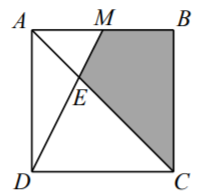
\includegraphics[width=\linewidth]{./cut_square-q00.png}
    \end{minipage}
    }{%
    Let $x$ be the side length of the square. $[AMD]=\frac{1}{4}x^2$ and $ADC=\frac{1}{2}x^2$. Let $F$ be the foot of the perpendicular from $E$ to $AD$. Because $AM:CD=1:2$, the height of $AME$ is $\frac{x}{3}$ so $FE$ is also $\frac{x}{3}$ and $[AED]=\frac{1}{6}x^2$
Now we get that $x^2-(\frac{1}{4}x^2+\frac{1}{2}x^2-\frac{1}{6}x^2)=400\implies x^2=\boxed{960}$
    }{%
    https://artofproblemsolving.com/community/c3t48f3h2700773_area_of_square_with_given_area_of_quadrilateral
}
